% Options for packages loaded elsewhere
\PassOptionsToPackage{unicode}{hyperref}
\PassOptionsToPackage{hyphens}{url}
%
\documentclass[
]{article}
\usepackage{amsmath,amssymb}
\usepackage{lmodern}
\usepackage{iftex}
\ifPDFTeX
  \usepackage[T1]{fontenc}
  \usepackage[utf8]{inputenc}
  \usepackage{textcomp} % provide euro and other symbols
\else % if luatex or xetex
  \usepackage{unicode-math}
  \defaultfontfeatures{Scale=MatchLowercase}
  \defaultfontfeatures[\rmfamily]{Ligatures=TeX,Scale=1}
\fi
% Use upquote if available, for straight quotes in verbatim environments
\IfFileExists{upquote.sty}{\usepackage{upquote}}{}
\IfFileExists{microtype.sty}{% use microtype if available
  \usepackage[]{microtype}
  \UseMicrotypeSet[protrusion]{basicmath} % disable protrusion for tt fonts
}{}
\makeatletter
\@ifundefined{KOMAClassName}{% if non-KOMA class
  \IfFileExists{parskip.sty}{%
    \usepackage{parskip}
  }{% else
    \setlength{\parindent}{0pt}
    \setlength{\parskip}{6pt plus 2pt minus 1pt}}
}{% if KOMA class
  \KOMAoptions{parskip=half}}
\makeatother
\usepackage{xcolor}
\usepackage[margin=1in]{geometry}
\usepackage{longtable,booktabs,array}
\usepackage{calc} % for calculating minipage widths
% Correct order of tables after \paragraph or \subparagraph
\usepackage{etoolbox}
\makeatletter
\patchcmd\longtable{\par}{\if@noskipsec\mbox{}\fi\par}{}{}
\makeatother
% Allow footnotes in longtable head/foot
\IfFileExists{footnotehyper.sty}{\usepackage{footnotehyper}}{\usepackage{footnote}}
\makesavenoteenv{longtable}
\usepackage{graphicx}
\makeatletter
\def\maxwidth{\ifdim\Gin@nat@width>\linewidth\linewidth\else\Gin@nat@width\fi}
\def\maxheight{\ifdim\Gin@nat@height>\textheight\textheight\else\Gin@nat@height\fi}
\makeatother
% Scale images if necessary, so that they will not overflow the page
% margins by default, and it is still possible to overwrite the defaults
% using explicit options in \includegraphics[width, height, ...]{}
\setkeys{Gin}{width=\maxwidth,height=\maxheight,keepaspectratio}
% Set default figure placement to htbp
\makeatletter
\def\fps@figure{htbp}
\makeatother
\setlength{\emergencystretch}{3em} % prevent overfull lines
\providecommand{\tightlist}{%
  \setlength{\itemsep}{0pt}\setlength{\parskip}{0pt}}
\setcounter{secnumdepth}{-\maxdimen} % remove section numbering
\newlength{\cslhangindent}
\setlength{\cslhangindent}{1.5em}
\newlength{\csllabelwidth}
\setlength{\csllabelwidth}{3em}
\newlength{\cslentryspacingunit} % times entry-spacing
\setlength{\cslentryspacingunit}{\parskip}
\newenvironment{CSLReferences}[2] % #1 hanging-ident, #2 entry spacing
 {% don't indent paragraphs
  \setlength{\parindent}{0pt}
  % turn on hanging indent if param 1 is 1
  \ifodd #1
  \let\oldpar\par
  \def\par{\hangindent=\cslhangindent\oldpar}
  \fi
  % set entry spacing
  \setlength{\parskip}{#2\cslentryspacingunit}
 }%
 {}
\usepackage{calc}
\newcommand{\CSLBlock}[1]{#1\hfill\break}
\newcommand{\CSLLeftMargin}[1]{\parbox[t]{\csllabelwidth}{#1}}
\newcommand{\CSLRightInline}[1]{\parbox[t]{\linewidth - \csllabelwidth}{#1}\break}
\newcommand{\CSLIndent}[1]{\hspace{\cslhangindent}#1}
\usepackage{authblk}
\author{Sara Cerioli$^1$}
\author{Andrey Formozov$^2$}
\affil{\small{$^1$Independent researcher, Mannheim, Germany \\
              $^2$Department of Neurophysiology, MCTN, Medical Faculty Mannheim, Heidelberg University,\\ 68167 Mannheim, Germany\\
       Correspondence: sara.cerioli@outlook.com, formozoff@gmail.com}}

\ifLuaTeX
  \usepackage{selnolig}  % disable illegal ligatures
\fi
\IfFileExists{bookmark.sty}{\usepackage{bookmark}}{\usepackage{hyperref}}
\IfFileExists{xurl.sty}{\usepackage{xurl}}{} % add URL line breaks if available
\urlstyle{same} % disable monospaced font for URLs
\hypersetup{
  pdftitle={A Refined Perspective on the Influence of Gender Equality on Gender Differences in Economic Preferences},
  hidelinks,
  pdfcreator={LaTeX via pandoc}}

\title{\textbf{A Refined Perspective on the Influence of Gender Equality
on Gender Differences in Economic Preferences}}
\author{}
\date{\vspace{-2.5em}}

\begin{document}
\maketitle

\hypertarget{methods}{%
\section{Methods}\label{methods}}

\hypertarget{overview}{%
\subsection{Overview}\label{overview}}

We replicate the results using the R programming language version 4.2.1
(2022-06-23), and its open-source IDE RStudio. The following packages
with respective versions are used:

Table:

\begin{longtable}[]{@{}lll@{}}
\toprule()
Package & \(\quad\) & Version \\
\midrule()
\endhead
data.table & & 1.14.2 \\
bit64 & & 4.0.5 \\
bit & & 4.0.5 \\
plyr & & 1.8.7 \\
dplyr & & 1.1.2 \\
haven & & 2.5.1 \\
ggplot2 & & 3.4.2 \\
missMDA & & 1.18 \\
MASS & & 7.3-58.1 \\
\bottomrule()
\end{longtable}

\hypertarget{data-collection-cleaning-and-standardization}{%
\subsection{Data Collection, Cleaning, and
Standardization}\label{data-collection-cleaning-and-standardization}}

\hypertarget{global-preferences-survey-and-gallup-world-poll-data-sets}{%
\subsubsection{Global Preferences Survey and Gallup World Poll data
sets}\label{global-preferences-survey-and-gallup-world-poll-data-sets}}

To download the GPS data set, one can go to the website of the Global
Preferences Survey
\href{https://www.briq-institute.org/global-preferences/home}{briq -
Institute on Behavior \& Inequality} in the section ``downloads''. The
data set is not provided in the rawest form: some variables were mixed
and already standardized. Some sociodemographic variables (for instance,
education level or income quintile) are not part of the Global
Preference Survey, but of the Gallup World Poll data set that is not
openly available. This data is protected by copyright and can not be
given to third parties. Check the website of the
\href{https://www.briq-institute.org/global-preferences/home}{briq -
Institute on Behavior \& Inequality} for more information on it.

\hypertarget{log-gdp-pc-and-gender-equality-indexes}{%
\subsubsection{Log GDP p/c and gender equality
indexes}\label{log-gdp-pc-and-gender-equality-indexes}}

From the \href{https://data.worldbank.org/indicator/}{website of the
World Bank}, one can access the data about the GDP per capita for a
certain set of years. The data for Log GDP p/c calculated in 2005 US
dollars was already archived. We used Log GDP p/c in 2010 US dollars
instead. To build an estimator for Log GDP p/c, we averaged the data
from 2003 until 2012 for all the available countries, as done in the
original article.

The Gender Equality Index used in the original article was composed of
four main data sets as the first component of the Principal Component
Analysis performed on them:

\begin{itemize}
\item
  \textbf{World Economic Forum Global Gender Gap Index:} Taken from the
  \href{http://reports.weforum.org/}{World Economic Forum Global Gender
  Gap Report 2015}. For countries where data was missing, data was added
  from the World Economic Forum Global Gender Gap Report 2006, as
  reported in the original article.
\item
  \textbf{United Nation Development Programme Gender Inequality Index:}
  Taken from the
  \href{http://hdr.undp.org/sites/default/files/hdr_2016_statistical_annex.pdf}{Human
  Development Report 2015}. We kept only the table called ``Gender
  Inequality Index''.
\item
  \textbf{Ratio of female and male labor force participation:} An
  average of estimates from 2004 to 2013 provided by the International
  Labor Organization in World Bank database
  (\url{http://data.worldbank.org/indicator/SL.TLF.CACT.FM.ZS}). Values
  were inverted to create an index of equality. Note that originally the
  data set was created taking the values between the years 2003 to 2012.
\item
  \textbf{Time since women's suffrage:} This indicator was build based
  on the data about the year of suffrage in a given country taken from
  the
  \href{http://www.ipu.org/wmn-e/suffrage.htm\#Note1}{Inter-Parliamentary
  Union Website}. For several countries more than one date where
  provided (for example, the right to be elected and the right to vote).
  We use the last date when both vote and stand for election rights were
  granted, with no other restrictions commented. Some countries were
  colonies or within a union of the countries (for instance, Kazakhstan
  in the Soviet Union). For these countries, the rights to vote and be
  elected might be technically granted two times within a union and as
  an independent state. In this case, we kept the first date. It was
  difficult to decide on South Africa because its history shows the
  racism part very entangled with women's rights (Walker 1990). We kept
  the latest date when also Black women could vote. For Nigeria,
  considering the distinctions between North and South, we decided to
  keep only the North data because, again, it was showing the
  completeness of the country and it was the last date.
\end{itemize}

In the extended analysis, we also involve the following index:

\begin{itemize}
\tightlist
\item
  \textbf{United Nation Development Programme Gender Development Index}
  taken from
  \href{https://hdr.undp.org/en/content/gender-development-index-gdi}{Human
  Development Reports 2020}. Note that we have downloaded the two tables
  of the Human Development Index for males and females, and used the
  ratio of the two as a GDI index, as described in the report.
\end{itemize}

\hypertarget{missing-data-and-imputation}{%
\subsubsection{Missing Data and
Imputation}\label{missing-data-and-imputation}}

One of the issues that we faced while trying to reproduce the results of
the article has been the missing data.

During the reproduction of the article, we found that the original
authors did not describe in detail how they handled missing data in the
indexes. They mention on page 14 of the Supplementary Material, that
(quoting): ``For countries where data were missing, data were added from
the World Economic Forum Global Gender Gap Report 2006
(\url{http://www3.weforum.org/docs/WEF_GenderGap_Report_2006.pdf}).''

However, regarding the year when women received the right to vote in a
specific country, the missing values are the ones coming from the United
Arab Emirates and Saudi Arabia, that neither in 2006 (when the WEF
Global Gender Gap Report that the authors quote as a reference for the
missing values) nor now (in 2022) have guaranteed the right to vote for
women yet. There is missing data also in the other sources that the
authors quote. So a quick search for the missing countries of the WEF
report of 2015, shows us that these countries can't be found in the
report of 2006 either. Missing data and imputation, in general, may not
be crucial for the replication of the analysis, although are not
desirable. The problem of missing data for a given country often does
not influence much the overall trends of found correlations. However, it
becomes very relevant for checking the implications of the study
concerning a specific country of interest.

\hypertarget{pure-replication-and-comparison-to-the-original-article}{%
\section{Pure replication and comparison to the Original
Article}\label{pure-replication-and-comparison-to-the-original-article}}

In this section, we describe how to reproduce the plots of FH and
compare their results to ours. Both simple linear regression (OLS) and
robust linear regression (RLR) were used.

\hypertarget{reproducing-the-figures-of-the-main-article}{%
\subsection{Reproducing the figures of the Main
Article}\label{reproducing-the-figures-of-the-main-article}}

To reproduce the plot of Figure 1A of the original article Falk \&
Hermle (2018a), we grouped the countries in quartiles based on the
logarithm of their average GDP p/c, extracted the mean of each
preference from the gender coefficients (the \(\beta_1^c\)) of the
countries for each quartile, after standardizing them. The same method
was applied to the GEI in correlation to gender differences for each
economic preference to reproduce the plot in Figure 1C of Falk \& Hermle
(2018a). Then, we related the magnitude of the summarized gender
difference coefficients (the first component of the PCA) with the
logarithm of the average GDP per capita to see the effect of economic
development. This reproduced Figure 1B of the original article. We used
a linear model to fit the correlation and extract the p-value. For the
plot the variables on the y-axis were additionally transformed as
\((y-y_{min})/(y_{max}-y_{min})\), as it was implemented in the original
article. We applied the same method to extract the correlation between
the GEI and the summarized gender preferences to see the effect of
gender equality (Figure 1D, of Falk \& Hermle (2018a)). Note that here
also the GEI is transformed to be on a scale between 0 and 1. It is
important to underline that such transformation may be misleading, as
GEI = 1 does not mean full gender equality (no country achieved this
state), and GEI = 0 does not necessarily represent the full absence of
it.

\begin{figure}
\centering
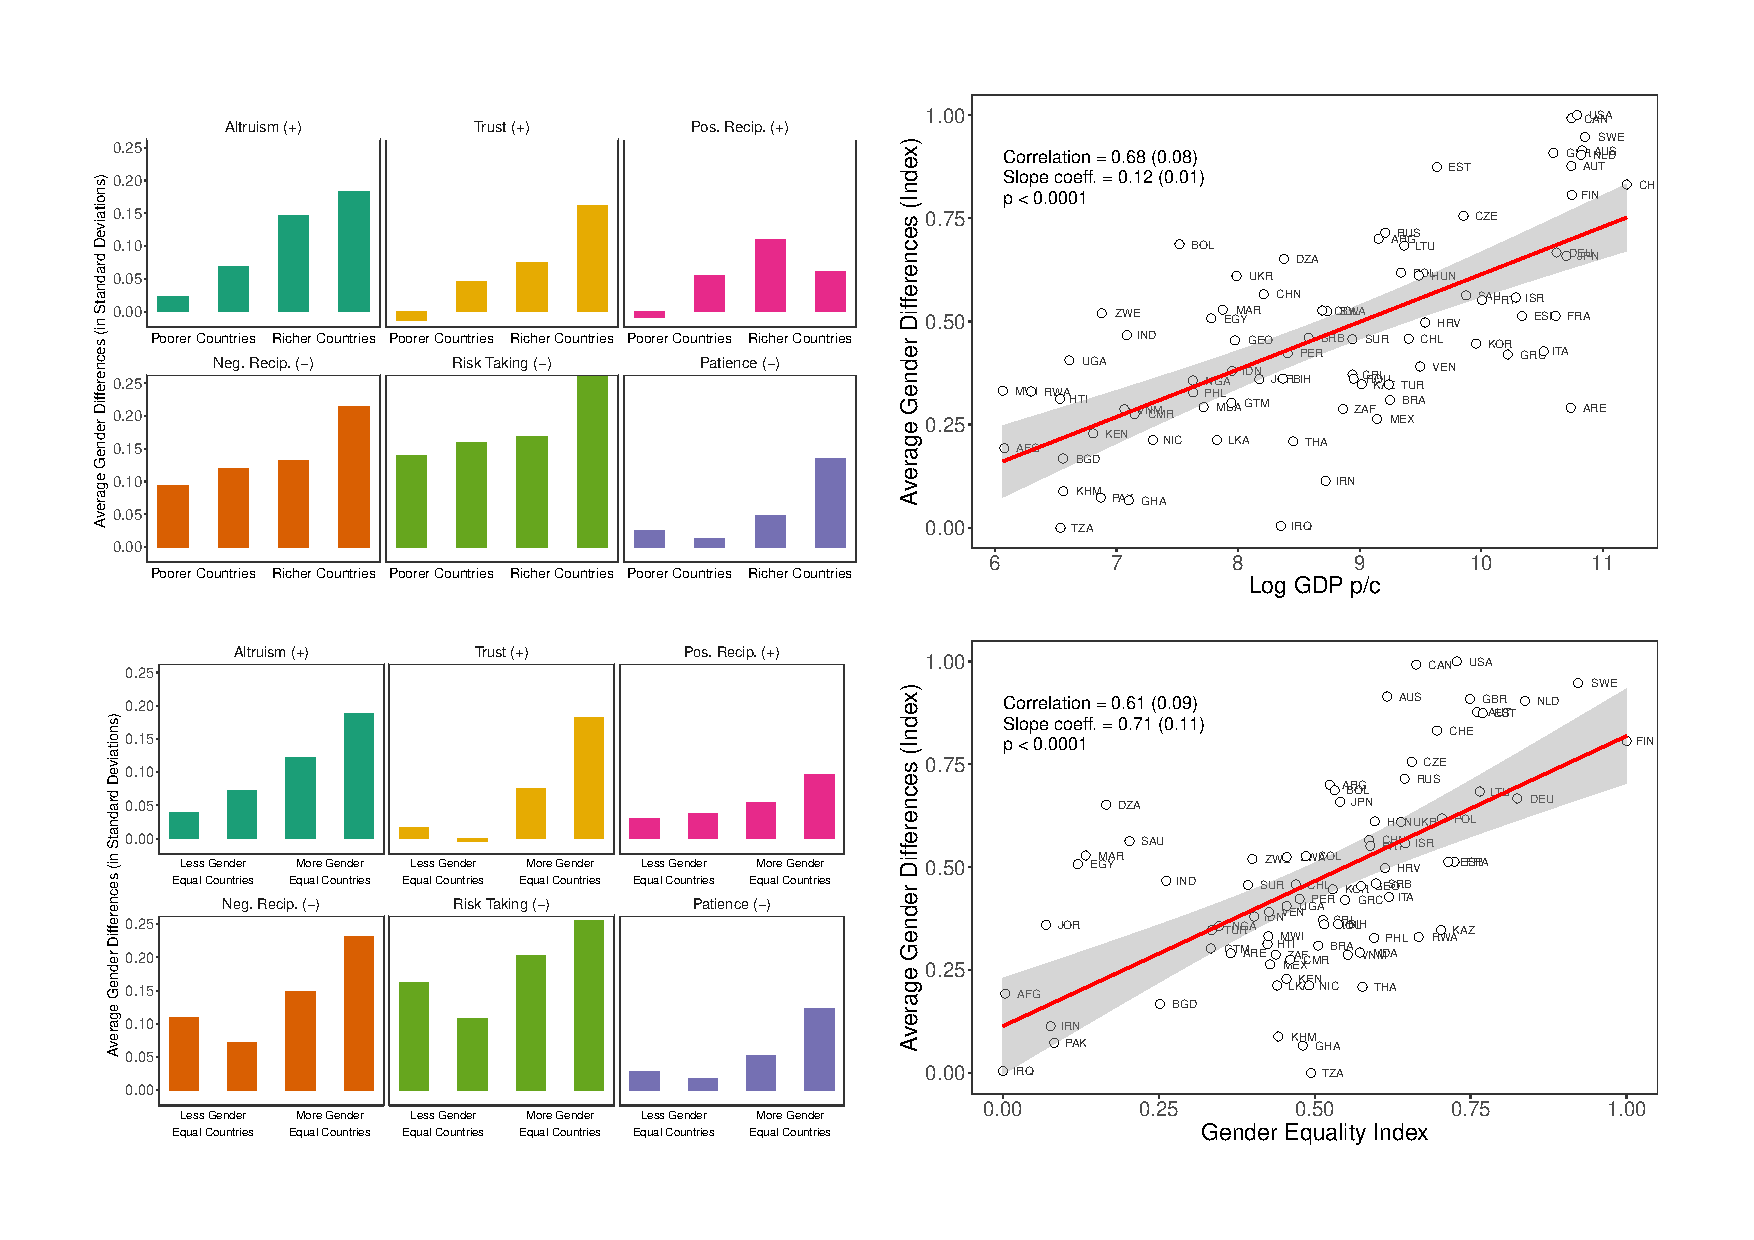
\includegraphics{figures/replication/main_Fig1.pdf}
\caption{Reproduction of the Fig 1 A-D of FH analysis. In the top left
figure, the countries were grouped by quartiles from poorer to richer,
and the standardized coefficient for the gender differences is plotted
for each of the individual economic preferences. Similarly, on the
bottom left, with less equal to more equal countries. On the right, the
correlation between gender differences in economic preferences
summarized into one single coefficient using the PCA, and economic
development (on top) and gender equality (bottom).}
\end{figure}

We summarized the results of Figure 1B and 1D in Table 2. Moreover, we
add in the same Table the results obtained using the RLR instead of the
OLS model.

\begin{longtable}[]{@{}
  >{\raggedright\arraybackslash}p{(\columnwidth - 6\tabcolsep) * \real{0.2500}}
  >{\raggedright\arraybackslash}p{(\columnwidth - 6\tabcolsep) * \real{0.2500}}
  >{\raggedright\arraybackslash}p{(\columnwidth - 6\tabcolsep) * \real{0.2500}}
  >{\raggedright\arraybackslash}p{(\columnwidth - 6\tabcolsep) * \real{0.2500}}@{}}
\caption{Correlation between PCA-summarized gender differences in
economic preferences vs Log GDP p/c and joint Gender Equality Index.
Significance \(\le\) 0.001 (***), \(\le\) 0.01 (**), \(\le\) 0.05
(*)}\tabularnewline
\toprule()
\begin{minipage}[b]{\linewidth}\raggedright
\end{minipage} & \begin{minipage}[b]{\linewidth}\raggedright
Original
\end{minipage} & \begin{minipage}[b]{\linewidth}\raggedright
Replication (OLS)
\end{minipage} & \begin{minipage}[b]{\linewidth}\raggedright
Replication (RLR)
\end{minipage} \\
\midrule()
\endfirsthead
\toprule()
\begin{minipage}[b]{\linewidth}\raggedright
\end{minipage} & \begin{minipage}[b]{\linewidth}\raggedright
Original
\end{minipage} & \begin{minipage}[b]{\linewidth}\raggedright
Replication (OLS)
\end{minipage} & \begin{minipage}[b]{\linewidth}\raggedright
Replication (RLR)
\end{minipage} \\
\midrule()
\endhead
Log GDP p/c & 0.6685*** & 0.68 (0.08)*** & 0.67 (0.09)*** \\
Gender Equality Index & 0.5580*** & 0.61 (0.09)*** & 0.59 (0.09)*** \\
\bottomrule()
\end{longtable}

We reproduced the plots in Figures 2A-F in Falk \& Hermle (2018a) using
the variable conditioning analysis (Figure 2). This has been done for
economic development, for the GEI, and for each of the four indexes
building the GEI. The variable used on the y-axis is the first Principal
Component of the PCA made on gender differences in the six preferences.
All the variables used have been standardized to have a mean at 0 and a
standard deviation of 1 before performing the conditional analysis.
Using the residuals, we performed a linear regression on the data points
and extracted correlation coefficients and p-values.

\begin{figure}
\centering
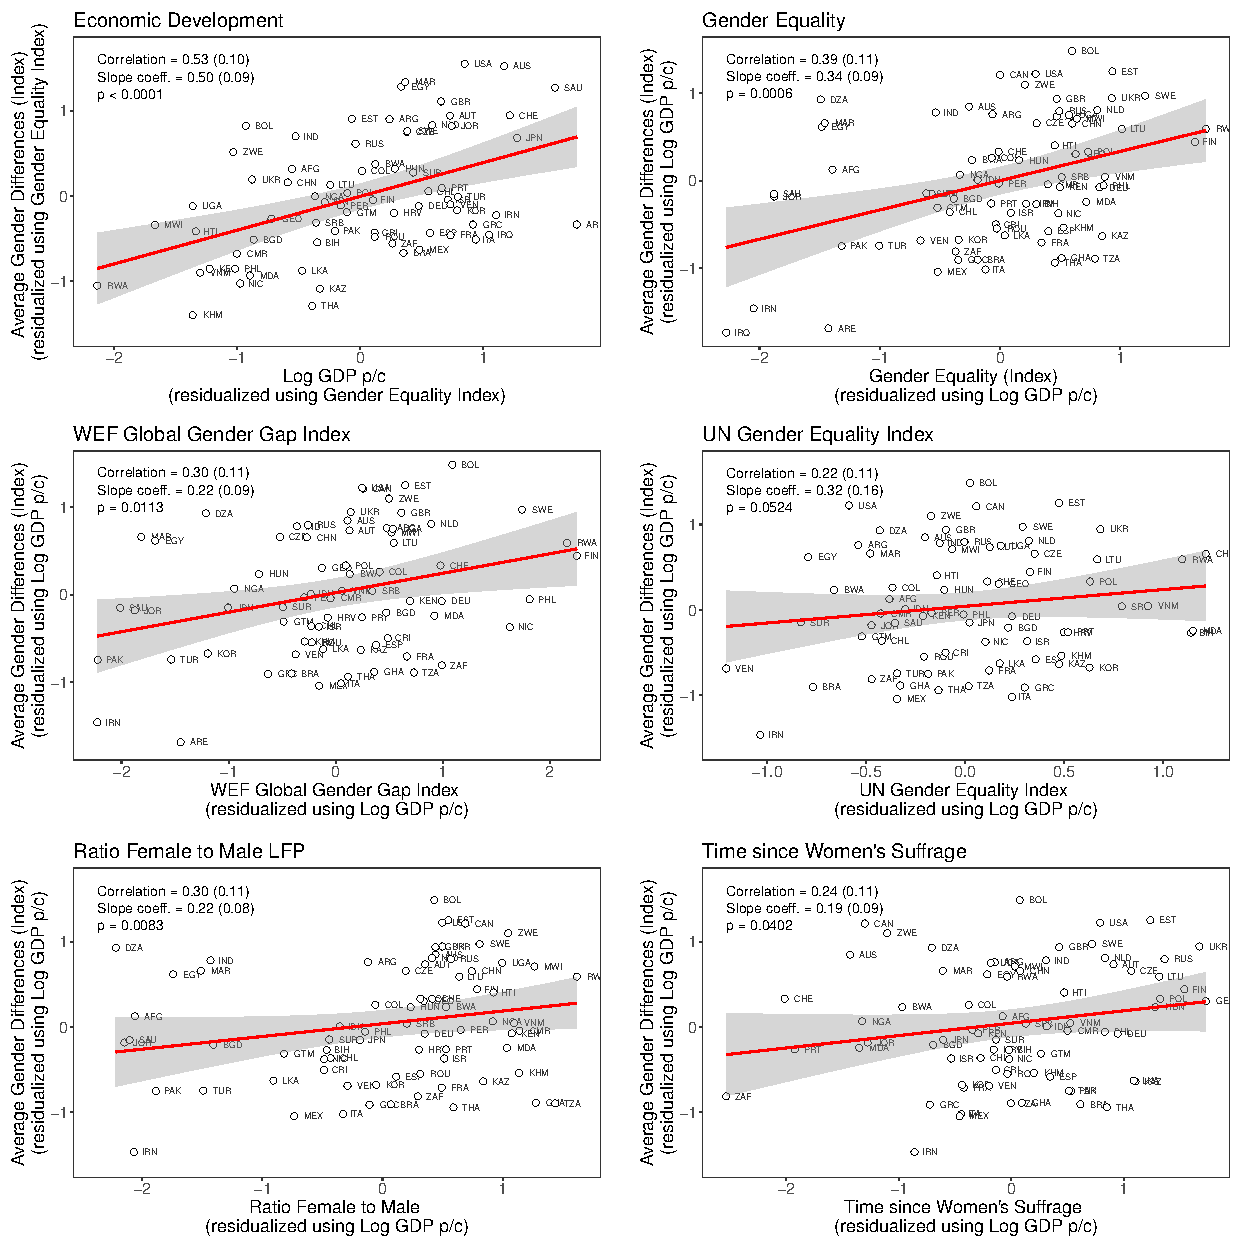
\includegraphics{figures/replication/main_Fig2.pdf}
\caption{Relationship between summarized gender differences in economic
preferences and economic development conditional on gender equality
(Figure 2A), and between summarized gender differences in economic
preferences and gender equality conditional on economic development,
with gender equality being represented by GEI (Fig 2B), by WEF GGGI
(Figure 2C), by UNDP GII (Figure 2D), by F/M LFP (Figure 2E), and by
TSWS (Figure 2F).}
\end{figure}

\hypertarget{correlation-between-economic-development-and-gender-equality}{%
\subsection{Correlation between Economic Development and Gender
Equality}\label{correlation-between-economic-development-and-gender-equality}}

As mentioned in our article, the fact that there is a correlation
between economic development and gender equality is revealed (Duflo
2012) and reported in the World Economic Forum (2015). We checked the
correlation between Log GDP p/c and GEI, reported here in Figure 3. In
addition, we checked the correlation of Log GDP p/c with the three
indexes used in our extended analysis for the measure of gender equality
(Figure 3): the WEF GGGI from the
\href{http://reports.weforum.org/}{World Economic Forum Global Gender
Gap Report 2015}, the UNDP GII
\href{http://hdr.undp.org/sites/default/files/hdr_2016_statistical_annex.pdf}{Human
Development Report 2015}, and the UNDP
\href{http://hdr.undp.org/en/indicators/137906}{Gender Development
Index} (GDI).

\begin{figure}
\centering
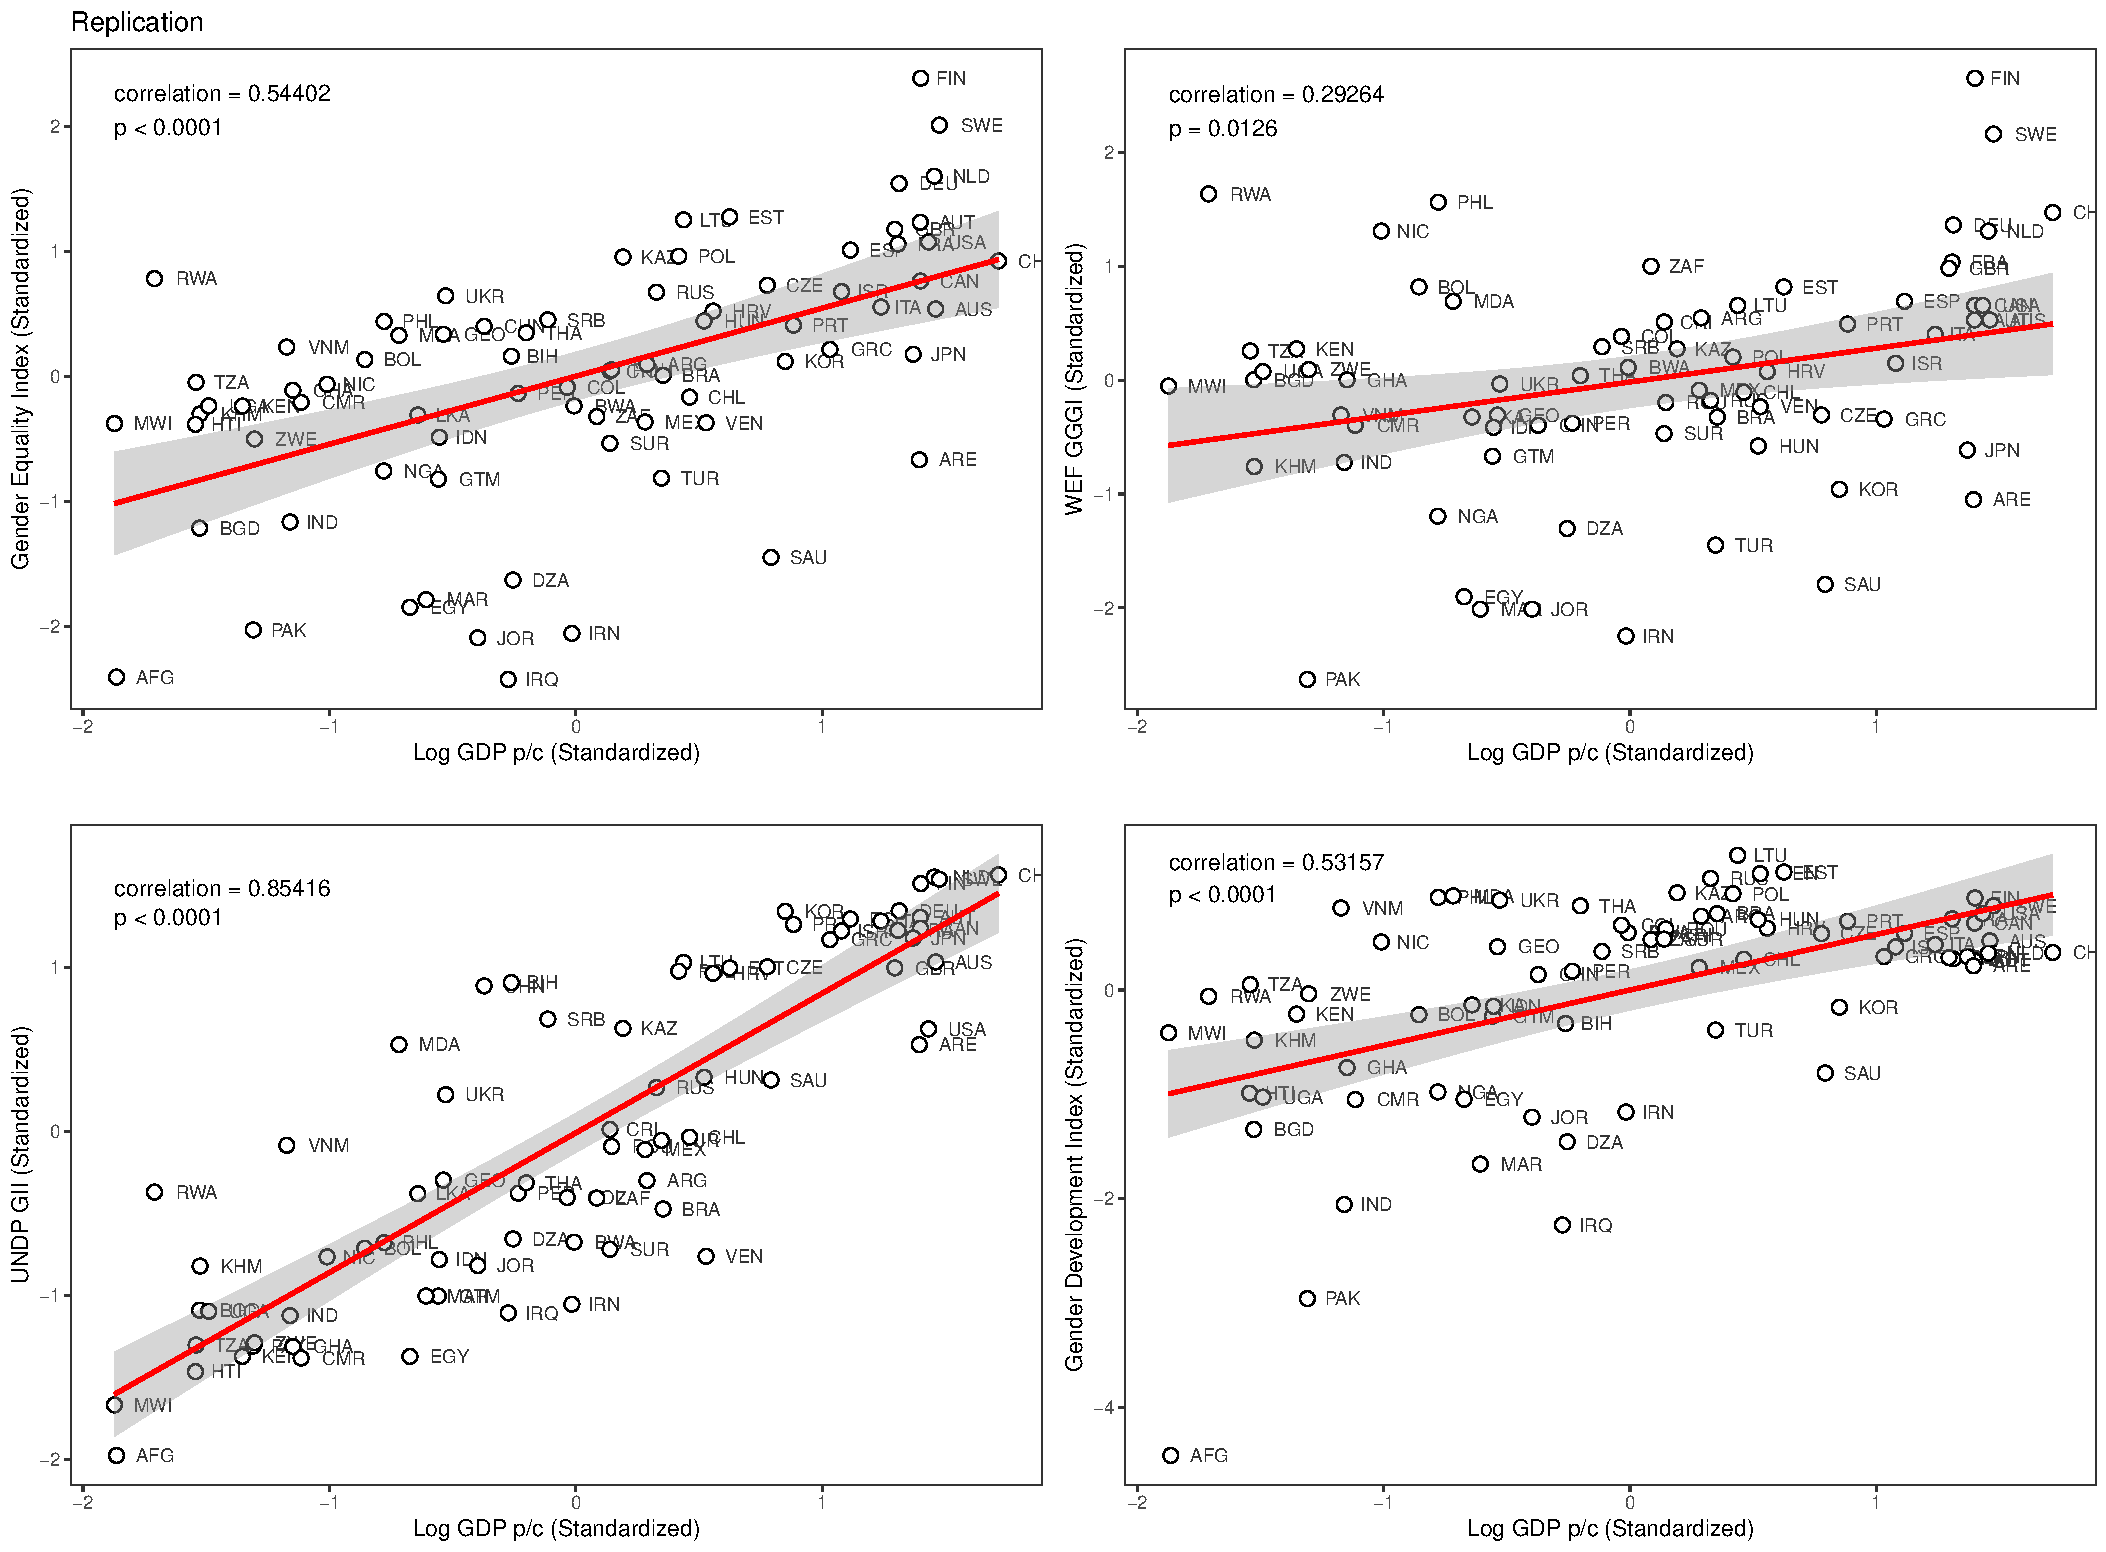
\includegraphics{figures/corr_equality_economicdev.pdf}
\caption{Correlation between gender equality indexes and economic
development by country. Note that only the countries that participated
in the original study are included.}
\end{figure}

\hypertarget{reproducing-the-results-in-fh-supplementary-material}{%
\subsection{Reproducing the results in FH Supplementary
Material}\label{reproducing-the-results-in-fh-supplementary-material}}

For the comparison of the results from Figure S4 in Falk \& Hermle
(2018b), we refer to Table 3, showing the correlation between the
average gender differences to the single-gender equality indexes. In
parenthesis, we put the standard deviation for the relative correlation
coefficient to have an overview of the level of agreement between the
original and the replication study. We report the replication results
using both the OLS and the RLR.

\begin{longtable}[]{@{}llll@{}}
\caption{Individual indexes for gender equality correlated with gender
differences in economic preferences. Significance \(\le\) 0.001 (***),
\(\le\) 0.01 (**), \(\le\) 0.05 (*)}\tabularnewline
\toprule()
& Original & Replication (OLS) & Replication (RLR) \\
\midrule()
\endfirsthead
\toprule()
& Original & Replication (OLS) & Replication (RLR) \\
\midrule()
\endhead
WEF GGGI & 0.4097*** & 0.41 (0.11)*** & 0.39 (0.11)** \\
UNDP GII & 0.6482*** & 0.67 (0.09)*** & 0.66 (0.09)*** \\
F/M LFP & 0.2661* & 0.29 (0.11)* & 0.26 (0.11)* \\
TSWS & 0.5139*** & 0.45 (0.10)*** & 0.45 (0.10)*** \\
\bottomrule()
\end{longtable}

For the comparison of the results of the Figure S5 and S6 of Falk \&
Hermle (2018b) to ours, refer to Table 4 and Table 5.

\begin{longtable}[]{@{}llll@{}}
\caption{Gender differences in single economic preferences regressed on
Log GDP p/c conditional on Gender Equality Index. Significance levels:
\(\le\) 0.001 (***), \(\le\) 0.01 (**), \(\le\) 0.05
(*).}\tabularnewline
\toprule()
& Original & Replication (OLS) & Replication (RLR) \\
\midrule()
\endfirsthead
\toprule()
& Original & Replication (OLS) & Replication (RLR) \\
\midrule()
\endhead
Trust & 0.4574*** & 0.43 (0.11)*** & 0.45 (0.10)*** \\
Altruism & 0.4751*** & 0.43 (0.10)*** & 0.40 (0.11)*** \\
Pos. Rec. & 0.2771* & 0.25 (0.11)* & 0.25 (0.11) \\
Neg. Rec. & 0.2444* & 0.21 (0.11) & 0.25 (0.11)* \\
Risk Tak. & 0.2868* & 0.23 (0.11) & 0.22 (0.11)* \\
Patience & 0.2621* & 0.23 (0.11)* & 0.24 (0.11)* \\
\bottomrule()
\end{longtable}

\begin{longtable}[]{@{}llll@{}}
\caption{Gender differences in single economic preferences regressed on
Gender Equality Index, conditional on Log GDP p/c.~Significance levels:
\(\le\) 0.001 (***), \(\le\) 0.01 (**), \(\le\) 0.05
(*).}\tabularnewline
\toprule()
& Original & Replication (OLS) & Replication (RLR) \\
\midrule()
\endfirsthead
\toprule()
& Original & Replication (OLS) & Replication (RLR) \\
\midrule()
\endhead
Trust & 0.2050 & 0.25 (0.11)* & 0.25 (0.11)* \\
Altruism & 0.3304** & 0.27 (0.11)* & 0.24 (0.11) \\
Pos. Rec. & -0.0115 & 0.05 (0.12) & 0.05 (0.12) \\
Neg. Rec. & 0.2788* & 0.22 (0.11) & 0.20 (0.11)* \\
Risk Tak. & 0.1973 & 0.19 (0.11) & 0.19 (0.11)* \\
Patience & 0.2967* & 0.28 (0.11)* & 0.28 (0.11)* \\
\bottomrule()
\end{longtable}

Lastly, we have reproduced the results from Figures S8 and S9 of Falk \&
Hermle (2018b) in Tables 6 and 7.

\begin{longtable}[]{@{}lll@{}}
\caption{Gender differences and economic development by preference using
preferences standardized at the global level. Economic preferences were
standardized at the global level, instead of using country level.
Significance levels: \(\le\) 0.001 (***), \(\le\) 0.01 (**), \(\le\)
0.05 (*).}\tabularnewline
\toprule()
& Original & Replication (OLS) \\
\midrule()
\endfirsthead
\toprule()
& Original & Replication (OLS) \\
\midrule()
\endhead
Trust & 0.5787*** & 0.58 (0.10)*** \\
Altruism & 0.5505*** & 0.59 (0.09)*** \\
Pos. Rec. & 0.2819* & 0.32 (0.11)** \\
Neg. Rec. & 0.2980** & 0.37 (0.11)** \\
Risk Tak. & 0.2974** & 0.36 (0.11)** \\
Patience & 0.4391*** & 0.41 (0.11)*** \\
\bottomrule()
\end{longtable}

\begin{longtable}[]{@{}lll@{}}
\caption{Gender differences and economic development by preference
without controls (OLS being performed using only gender as a independent
variable). Significance levels: \(\le\) 0.001 (***), \(\le\) 0.01 (**),
\(\le\) 0.05 (*).}\tabularnewline
\toprule()
& Original & Replication (OLS) \\
\midrule()
\endfirsthead
\toprule()
& Original & Replication (OLS) \\
\midrule()
\endhead
Trust & 0.5434*** & 0.55 (0.10)*** \\
Altruism & 0.5808*** & 0.59 (0.09)*** \\
Pos. Rec. & 0.2748* & 0.28 (0.11)* \\
Neg. Rec. & 0.4038*** & 0.39 (0.11)*** \\
Risk Tak. & 0.3860*** & 0.39 (0.11)*** \\
Patience & 0.4830*** & 0.48 (0.10)*** \\
\bottomrule()
\end{longtable}

\hypertarget{further-notes-on-the-replication}{%
\subsubsection{Further notes on the
replication}\label{further-notes-on-the-replication}}

The Figure S7 of Falk \& Hermle (2018b) could not be replicated because
there is no access to raw data. For the replication of several tables in
the supplementary material, the description of the data sets and the
analysis approach was not sufficient for replication.

\hypertarget{references}{%
\section*{References}\label{references}}
\addcontentsline{toc}{section}{References}

\hypertarget{refs}{}
\begin{CSLReferences}{1}{0}
\leavevmode\vadjust pre{\hypertarget{ref-10.2307ux2f23644911}{}}%
Duflo, E. (2012). Women empowerment and economic development.
\emph{Journal of Economic Literature}, \textbf{50}, 1051--1079.
Retrieved from \url{http://www.jstor.org/stable/23644911}

\leavevmode\vadjust pre{\hypertarget{ref-doi:10.1126ux2fscience.aas9899}{}}%
Falk, A. \& Hermle, J. (2018a). Relationship of gender differences in
preferences to economic development and gender equality. \emph{Science},
\textbf{362}, eaas9899. Retrieved from
\url{https://www.science.org/doi/abs/10.1126/science.aas9899}

\leavevmode\vadjust pre{\hypertarget{ref-FH_SM}{}}%
Falk, A. \& Hermle, J. (2018b).
\href{http://science.sciencemag.org/content/suppl/2018/10/17/362.6412.eaas9899.DC1}{Supplementary
materials of {R}elationship of gender differences in preferences to
economic development and gender equality}.

\leavevmode\vadjust pre{\hypertarget{ref-SAHO}{}}%
Walker, C. (1990). Women and gender in southern {A}frica to 1945.
Retrieved from
\url{https://www.sahistory.org.za/archive/womens-suffrage-movement-politics-gender-race-and-class-cheryl-walker}

\leavevmode\vadjust pre{\hypertarget{ref-GGGreport2015}{}}%
World Economic Forum. (2015). {G}lobal {G}ender {G}ap report 2015.
Retrieved from
\url{https://reports.weforum.org/global-gender-gap-report-2015/the-global-gender-gap-index-2015/}

\end{CSLReferences}

\end{document}
